% TODO: Commento intervalli di confidenza
% TODO: rileggere la parte relativa ai risultati ottenuti
% TODO: rilettura
% TODO: commento sul migliore modello
% TODO: Commento sugli intervalli di confidenza in relazione agli altri modelli
% TODO: Confronto con il percettrone
\chapter{Rete neurale} \label{chp:reteNeurale}
La fase di analisi presentata nella sezione \ref{sec:analisi-descrittiva} ha
permesso di acquisire informazioni utili sulla struttura del dataset e di
conseguenza permettere la selezione di un modello adatto a svolgere il compito
di classificazione.

In questo capitolo verrà presentato uno dei tre modelli che sono stati realizzati
per svolgere il compito di classificazione, ovvero la \textbf{rete neurale}. Nello
specifico, in questo capitolo si andranno a presentare i passaggi che sono stati
effettuati per la realizzazione di questo modello, partendo dalla preparazione
dei dati, passando per la definizione della struttura della rete neurale, fino
ad arrivare ai risultati ottenuti. In un secondo momento, si andranno a
confrontare i risultati ottenuti con quelli ottenuti da un modello addestrato
con PCA.
\section{Preparazione dei dati}
Prima di passare alla presentazione della rete neurale nel dettaglio, è importante
delineare il processo di preparazione dei dati necessario per l'addestramento
della stessa.

La preparazione dei dati è stata eseguita attraverso una serie di operazioni
mirate a renderli idonei per l'addestramento della rete neurale. Le fasi
principali sono state le seguenti:
\begin{itemize}
    \item \textbf{Standardizzazione dei dati}: Ogni caratteristica è stata
          trasformata in modo tale che la loro media fosse pari a 0 e la
          deviazione standard fosse 1. Questo passaggio è stato cruciale per
          garantire che la rete neurale non fosse influenzata da valori di input
          su differenti scale.
    \item \textbf{Suddivisione del dataset in training set e test set}: Il
          dataset è stato diviso in due parti: il training set e il test set.
          Questo processo è stato fondamentale per valutare le prestazioni della
          rete neurale su dati non utilizzati durante la fase di addestramento.
          Il training set ha rappresentato l'$80\%$ dei dati, mentre il test
          set il restante $20\%$.
\end{itemize}
Essendo il dataset non perfettamente bilanciato ($55\%$ dati negativi e $45\%$
dati positivi) l'operazione di suddivisione è stata effettuata in modo da
mantenere la stessa percentuale di dati positivi e negativi in entrambi i set.
Lo scopo di questa scelta è quello di evitare che il modello sia addestrata su
un dataset sbilanciato e di conseguenza non sia in grado di generalizzare
correttamente.
\section{Struttura della rete neurale}
La fase di definizione della struttura della rete neurale è stata effettuata
attraverso una serie di passaggi. Inizialmente, è stata effettuata un'analisi
dei dati in modo tale da selezionare un sottoinsieme di feature le quali sono
state utilizzate come input della rete neurale. Questo sottoinsieme è stato
selezionato in modo tale da garantire che la rete neurale fosse in grado di
discriminare in modo efficace le due classi.

In seguito, è stata effettuata una fase di grid search per valutare la combinazione
migliore di iperparametri per la rete neurale. Questa fase è stata effettuata
attraverso una cross validation a 5 fold, prendendo in considerazione solamente
i dati del training set.

Dai risultati ottenuti dalla fase di analisi e dal dominio del problema, si è
scelto di utilizzare una rete con una struttura di dimensioni ridotte, in modo
tale da ridurre le possibilità che la rete neurale soffra di overfitting.

Per svolgere il compito di classificazione si è scelto di utilizzare una rete
neurale feedforward, la cui struttura, a meno del layer di input e di output, è
stata definita attraverso il processo di grid search.
\subsection{Ottimizzazione degli iperparametri}
Come già accennato in precedenza, la ricerca degli iperparametri della rete neurale
è stata effettuata attraverso un processo di grid search. Questo processo ha
permesso di valutare le prestazioni della rete neurale al variare della funzione
di attivazione, del numero di layer nascosti e del numero di neuroni per ogni
layer nascosto.

Visti i risultati ottenuti nella fase di analisi e la volontà di mantenere i
tempi di addestramento bassi, si è scelto di mantenere una struttura di dimensioni
ridotte per la rete neurale. Per questo motivo, l'operazione di grid search è
stata effettuata prendendo in considerazione un numero di neuroni per layer
tra 5, 10 mentre il numero di layer nascosti è stato valutato tra 1 e 2.

Per quanto riguarda la funzione di attivazione, sono state valutate le seguenti
funzioni di attivazione:
\begin{itemize}
    \item \textit{ReLU}
    \item \textit{Leaky ReLU}
    \item \textit{sigmoid}
\end{itemize}

\begin{figure}[!ht]
    \centering
    \begin{subfigure}[b]{0.3\textwidth}
        \centering
        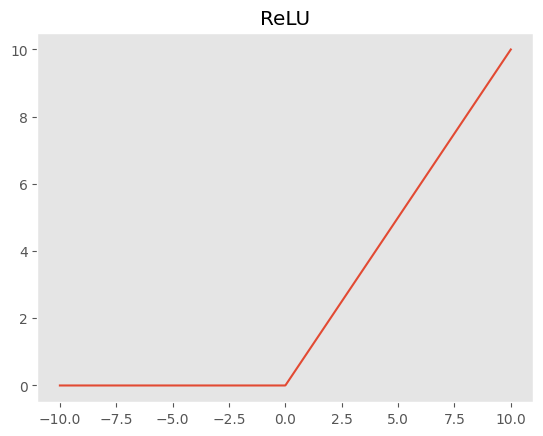
\includegraphics[width=\textwidth]{img/rete/relu.png}
        \caption{ReLU}
        \label{fig:relu}
    \end{subfigure}
    \hfill
    \begin{subfigure}[b]{0.3\textwidth}
        \centering
        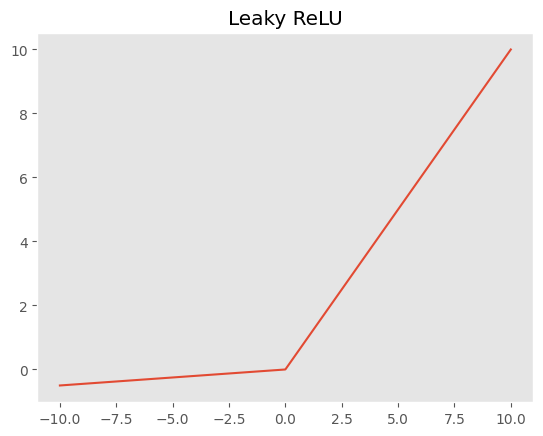
\includegraphics[width=\textwidth]{img/rete/leaky_relu.png}
        \caption{Leaky ReLU}
        \label{fig:leaky-relu}
    \end{subfigure}
    \hfill
    \begin{subfigure}[b]{0.3\textwidth}
        \centering
        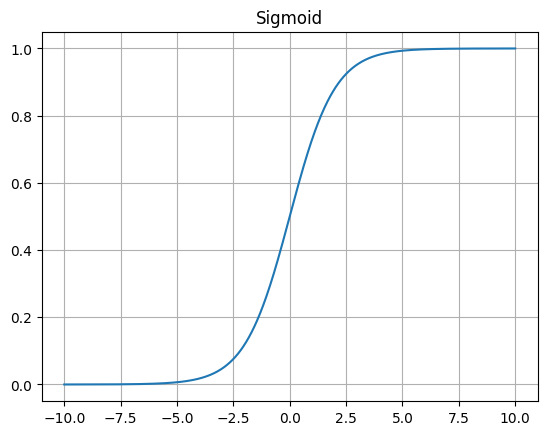
\includegraphics[width=\textwidth]{img/rete/sigmoid.png}
        \caption{Sigmoide}
        \label{fig:sigmoid}
    \end{subfigure}
    \caption{Funzioni di attivazione utilizzate nella fase di grid search}
    \label{fig:}
\end{figure}

Durante il processo di grid search, per ogni modello che è stato addestrato, sono
state raccolte delle informazioni relative all'accuratezza, al tempo di addestramento
richiesto. In aggiunta a queste informazioni, dato che ogni modello è stato
addestrato attraverso una cross validation a 5 fold, sono stati calcolati gli
intervalli di confidenza al $90\%$ per ogni modello addestrato.

Ottenuti i risultati, si è proceduto con l'analisi di questi, in modo tale da
definire la struttura della rete neurale. Per effettuare questa valutazione sono
state utilizzate le misure precedentemente citate.

Il modello selezionato è stato scelto in base al seguente criterio:
\begin{center}
    \textit{Modello = 2 * Accuratezza + 2 * Tempo di addestramento + 1 * Intervalli di confidenza}
\end{center}
Le misure di accuratezza e tempo di addestramento si riferiscono alla media
calcolata attraverso la cross validation.

Nello specifico, sono stati utilizzati i seguenti pesi: 2 per l'accuratezza
media, 2 per il tempo di addestramento medio e 1 per gli intervalli di
confidenza. Questi pesi sono stati scelti in modo tale da dare più importanza
all'accuratezza media e al tempo di addestramento medio, in quanto sono le due
misure che permettono di valutare le prestazioni della rete neurale, mentre gli
intervalli di confidenza sono stati utilizzati per valutare la variabilità delle
prestazioni.

Per verificare la validità del modello scelto si è proceduto con il confronto di
esso con la rete che ha ottenuto la migliore accuratezza e quella che ha ottenuto
il tempo di addestramento minore, ottenendo i risultati riportati in tabella \ref{tab:ris-grid-search}.
\begin{table}[ht]
    \centering
    \begin{tabular}{@{}lcc@{}}
        \toprule
        \rowcolor[HTML]{EFEFEF}
        \multicolumn{1}{c}{\cellcolor[HTML]{EFEFEF}\textbf{Modello}} & \textbf{Accuratezza} & \textbf{Tempo di addestramento} \\ \midrule
        Tempo di addestramento minore                                & 97.9\%               & 1.05s                           \\
        Accuratezza maggiore                                         & 99.0\%               & 14.43s                          \\
        Modello scelto                                               & 98.6\%               & 2.59s                           \\ \bottomrule
    \end{tabular}
    \caption{Risultati ottenuti dalla fase di grid search}
    \label{tab:ris-grid-search}
\end{table}

Dai valori riportati nella tabella \ref{tab:ris-grid-search} si può notare che il
notare che il modello che è stato selezionato fornisce un compromesso tra
accuratezza e tempo di addestramento. Nello specifico, perdendo lo $0.4\%$ di
accuratezza si è ottenuto un tempo di addestramento minore di circa $12$ secondi.
\subsection{Definizione della struttura della rete neurale}
Dalla fase di analisi è stato selezionato un sottoinsieme di feature le quali
sono state utilizzate come input della rete neurale. Questo sottoinsieme è
composto da 5 elementi, il che ha permesso di definire la struttura del layer di
input della rete neurale, questo primo strato è composto da 5 neuroni, uno per 
ogni feature selezionata.

I risultati ottenuti dalla fase di grid search hanno permesso di definire la
struttura della rete neurale. In particolare, la rete neurale è composta da 1
layer di input, 2 layer nascosti e 1 layer di output.

I layer nascosti sono composti nel seguente modo:
\begin{itemize}
    \item Il primo layer nascosto è composto da 10 neuroni, in cui la funzione di
          attivazione è la funzione ReLU \ref{fig:relu}.
    \item Il secondo layer nascosto è composto da 5 neuroni, in cui la funzione
          di attivazione è la funzione ReLU \ref{fig:relu}.
\end{itemize}

Per concludere la descrizione della struttura della rete neurale, è necessario
specificare come è composto l'ultimo layer, ovvero quello di output. Vista la
natura del problema di classificazione, il layer di output è composto da un solo
neurone, in cui la funzione di attivazione è la funzione sigmoide \ref{fig:sigmoid}.
\begin{equation}
    \sigma(x) = \frac{1}{1 + e^{-x}}
\end{equation}
Questa scelta è dovuta al fatto che tale funzione restituisce un valore compreso
tra 0 e 1, il che permette di interpretare l'output della rete neurale come la
probabilità che l'input appartenga alla classe positiva.

La struttura della rete neurale è riassunta nella figura \ref{fig:strutturaReteNeurale}.
\begin{figure}[!ht]
    \centering
    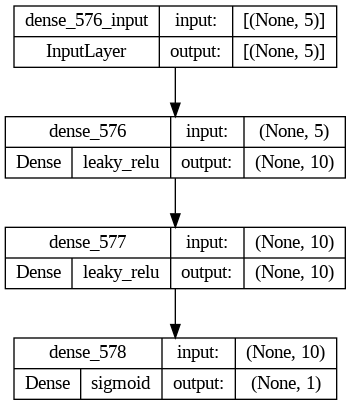
\includegraphics[width=0.3\textwidth]{img/rete/struttura_rete.png}
    \caption{Struttura della rete neurale}
    \label{fig:strutturaReteNeurale}
\end{figure}
\subsection{Altri iperparametri} % TODO: titolo migliore
Oltre alla ricerca della struttura della rete neurale, la fase di grid search è
stata utilizzata per valutare l'algoritmo di ottimizzazione, il numero di epoche
e la dimensione del batch.

Per quanto riguarda l'algoritmo di ottimizzazione, il confronto è stato eseguito
tra \textit{Adam} e \textit{SGD}, mentre per il numero di epoche e la dimensione
del batch sono stati valutati i valori 100, 300 per il numero di epoche e 50,
100, 300 per la dimensione del batch.

I risultati ottenuti dalla fase di grid search hanno permesso di definire i valori
degli iperparametri che hanno permesso di ottenere i migliori risultati. In
particolare, l'algoritmo di ottimizzazione scelto è \textit{Adam}, mentre il
numero di epoche e la dimensione del batch sono stati impostati a 100 e 100
rispettivamente.

In questa fase è stato necessario definire la funzione di perdita. Si è scelta
la \textit{binary crossentropy} in quanto adatta a problemi di classificazione
binaria. La scelta di questa loss è dovuta alla natura del problema di
classificazione che si vuole risolvere.
\section{Addestramento della rete neurale}
La fase di addestramento della rete neurale è stata effettuata utilizzando il
training set precedentemente definito. L'addestramento della rete neurale è stato
effettuato utilizzando la libreria \textit{Keras} in quanto permette di definire
e addestrare reti neurali in modo intuitivo.
\section{Risultati}
Vista il dominio del problema, ovvero la classificazione di dati medici, si è
deciso di modificare manualmente il valore della soglia per la predizione
del tumore. Questa scelta è stata fatta in quanto si è voluto ridurre al minimo
il numero di falsi negativi, ovvero il numero di casi in cui il modello predice
l'assenza di tumore quando in realtà è presente.

Per realizzare questa operazione si è scelto di impostare il valore di threshold
a $0.3$, in modo tale da ridurre il numero di falsi negativi. Questa scelta è
stata fatta in quanto si è voluto dare più importanza al valore di richiamo, il
quale permette di valutare la capacità del modello di individuare i veri positivi.

Fatta questa precisazione, si può procedere con la presentazione dei risultati
ottenuti. Utilizzando i dati del test set, è stato possibile valutare le
prestazioni della rete neurale addestrata. In particolare, sono state calcolate
le seguenti metriche:
\begin{itemize}
    \item Accuratezza
    \item Precisione
    \item Richiamo
    \item F1 score
\end{itemize}
Oltre al calcolo di queste metriche, si è deciso di realizzare la curva ROC per
il modello e di rappresentare la matrice di confusione. Nella tabella
\ref{tab:risultatiReteNeurale} sono presentati i risultati ottenuti dal modello
addestrato.
\begin{table}[!ht]
    \centering
    \begin{tabular}{@{}cllll@{}}
        \toprule
        \rowcolor[HTML]{EFEFEF}
        \textbf{Metrica}                        & \textbf{Accuratezza}         & \textbf{Precisione}          & \textbf{Richiamo}            & \textbf{F1 score}            \\ \midrule
        \cellcolor[HTML]{EFEFEF}\textbf{Valore} & \multicolumn{1}{c}{98.93 \%} & \multicolumn{1}{c}{98.52 \%} & \multicolumn{1}{c}{99.10 \%} & \multicolumn{1}{c}{98.81 \%} \\ \bottomrule
    \end{tabular}
    \caption{Risultati ottenuti dal modello addestrato}
    \label{tab:risultatiReteNeurale}
\end{table}

Dai valori riportati nella tabella \ref{tab:risultatiReteNeurale} si può notare
che la rete neurale ha ottenuto dei valori delle metriche molto alti. Questo
comportamento è giustificato dal fatto che in fase di analisi è stato possibile
notare che le feature selezionate sono in grado di discriminare in modo efficace
le due classi.

In aggiunta al calcolo di queste metriche, è stata calcolata la matrice di confusione
per il modello addestrato. La matrice di confusione ottenuta è riportata in figura
\ref{fig:matriceConfusioneReteNeurale}.

\begin{figure}[!ht]
    \centering
    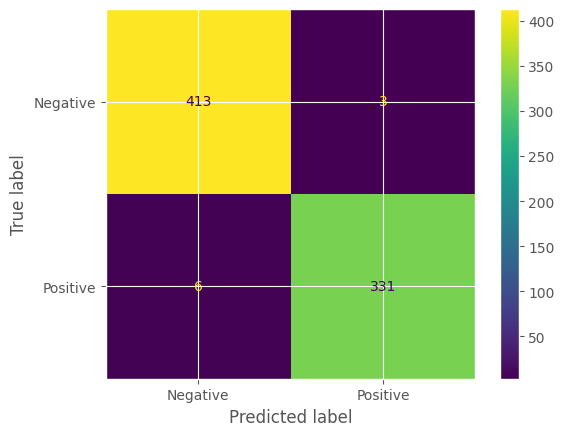
\includegraphics[width=0.5\textwidth]{img/rete/matrice_confusione.png}
    \caption{Matrice di confusione ottenuta dal modello addestrato}
    \label{fig:matriceConfusioneReteNeurale}
\end{figure}

Dalla matrice di confusione è possibile confermare i risultati ottenuti dalle
metriche calcolate in precedenza. Inoltre, avendo corretto manualmente il valore
della soglia, si è riusciti a ridurre il numero di falsi negativi, il che ha
permesso di aumentare il valore del richiamo.

Per concludere questa prima parte di analisi dei risultati, è stata realizzata
la curva ROC per il modello addestrato. La curva ROC ottenuta è riportata in
figura \ref{fig:curvaRocReteNeurale}. Oltre alla curva ROC è stata calcolata
l'area sotto la curva, la quale ha ottenuto un valore di $1.00$. Questo valore
ci permette di affermare che il modello addestrato si avvicina molto alla
perfetta classificazione.

\begin{figure}[!ht]
    \centering
    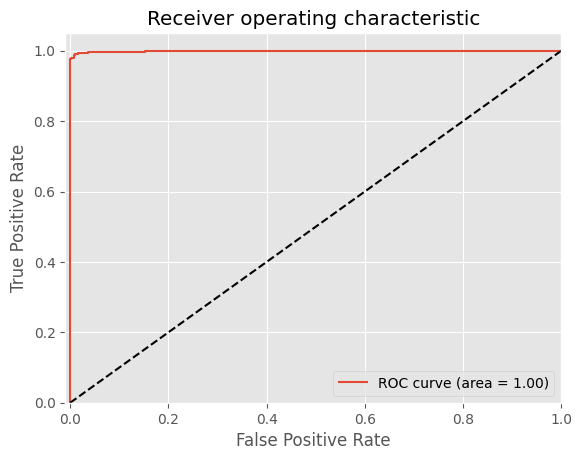
\includegraphics[width=0.8\textwidth]{img/rete/curva_roc.png}
    \caption{Curva ROC ottenuta dal modello addestrato}
    \label{fig:curvaRocReteNeurale}
\end{figure}
\subsection*{K-fold validation}
Per avere una visione più chiara dei risultati ottenuti, si è deciso di effettuare
una valutazione del modello attraverso 10 fold di cross validation. In questo
processo ogni modello che è stato addestrato è stato valutato attraverso le
metriche di accuratezza, precisione, richiamo e F1 score.

Per svolgere questa operazione è stato utilizzato il dataset completo, ovvero
senza alcuna suddivisione in training set e test set.

Anche per questa operazione è stato utilizzato il valore di threshold precedentemente
definito, ovvero $0.3$.

Sui risultati ottenuti da questo processo sono stati calcolati gli intervalli
di confidenza al $90\%$. I risultati ottenuti sono riportati in tabella
\ref{tab:risultatiCrossValidation}.

\begin{table}[ht]
    \centering
    \begin{tabular}{@{}lcc@{}}
        \toprule
        \rowcolor[HTML]{EFEFEF}
        \multicolumn{1}{c}{\cellcolor[HTML]{EFEFEF}\textbf{Metrica}} & \textbf{Valore Medio} & \textbf{Intervallo di confidenza} \\ \midrule
        Accuratezza                                                  & 98.27 \%              & [97.98\%, 98.55\%]                \\
        Precisione                                                   & 97.99 \%              & [97.47\%, 98.52\%]                \\
        Richiamo                                                     & 98.15 \%              & [97.49\%, 98.81\%]                \\
        F1 score                                                     & 98.06 \%              & [97.75\%, 98.38\%]                \\ \bottomrule
    \end{tabular}
    \caption{Risultati ottenuti dalla cross validation}
    \label{tab:risultatiCrossValidation}
\end{table}

Gli intervalli ottenuti sono stati successivamente rappresentati in un grafico
riportato in figura \ref{fig:risultatiCrossValidation}. Questo grafico permette
di avere una visione più chiara dei risultati ottenuti dalla cross validation.

\begin{figure}[!ht]
    \centering
    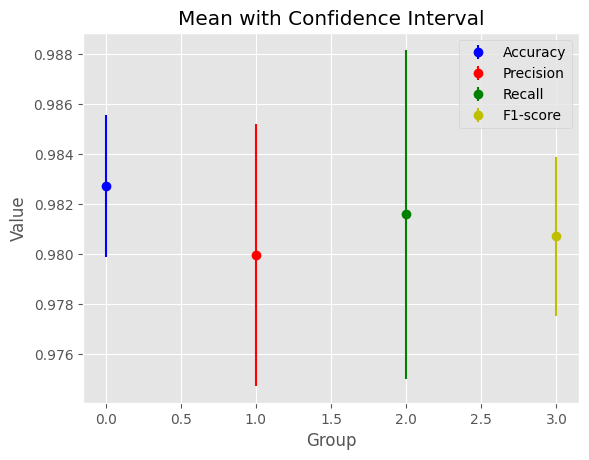
\includegraphics[width=0.5\textwidth]{img/rete/intervalli_confidenza.png}
    \caption{Risultati ottenuti dalla cross validation}
    \label{fig:risultatiCrossValidation}
\end{figure}
\section{Modello addestrato con PCA}
Per verificare se i risultati ottenuti dal modello addestrato sulle feature da
noi selezionate siano effettivamente dovuti alla struttura delle feature e non
a una fortunata selezione, si è deciso di addestrare un modello con le feature
ottenute attraverso la PCA.

Il dataset ottenuto attraverso la PCA, descritto sella sezione \ref{sec:pca}, è
stato diviso in training set e test set in modo tale da mantenere la stessa
percentuale di dati positivi e negativi in entrambi i set. Oltre a questa
operazione, i dati sono stati standardizzati.
\subsection{Struttura}
Come per il modello addestrato con le feature selezionate manualmente, anche per
questo modello è stata effettuata una fase di grid search per valutare la
combinazione migliore di iperparametri per la rete neurale.

Il processo utilizzato in questa fase è analogo a quello utilizzato per il modello
precedente, sia a livello di iperparametri che di valutazione del modello.

Come fatto in precedenza, il modello selezionato è stato confrontato con il modello
che ha ottenuto la migliore accuratezza e quello che ha ottenuto il tempo di
addestramento minore. I risultati ottenuti sono riportati in tabella \ref{tab:ris-grid-search-pca}.

\begin{table}[ht]
    \centering
    \begin{tabular}{@{}lcc@{}}
        \toprule
        \rowcolor[HTML]{EFEFEF}
        \textbf{Modello}              & \textbf{Accuratezza} & \textbf{Tempo di addestramento} \\ \midrule
        Tempo di addestramento minore & 96.9\%               & 1.06s                           \\
        Accuratezza maggiore          & 98.0\%               & 22.20s                          \\
        Modello scelto                & 97.9\%               & 1.16s                           \\ \bottomrule
    \end{tabular}
    \caption{Risultati ottenuti dalla fase di grid search}
    \label{tab:ris-grid-search-pca}
\end{table}
Anche in questo caso, come per il precedente, il modello che è stato selezionato
rappresenta un compromesso tra accuratezza e tempo di addestramento. In particolare,
perdendo lo $0.1\%$ di accuratezza si è ottenuto un tempo di addestramento minore
di circa $21$ secondi.


I risultati ottenuti dalla fase di grid search hanno permesso di definire la
struttura della rete neurale. In particolare, la rete neurale è composta da 1
layer di input, 1 layer nascosto e 1 layer di output.

Il layer di input è composto da 3 neuroni, uno per ogni componente principale
ottenuta attraverso la PCA. Questo primo strato è stato definito in questo modo
in quanto il dataset ottenuto attraverso la PCA è composto da 3 feature.

Il layer nascosto è composto da 10 neuroni, in cui la funzione di attivazione è
la funzione ReLU \ref{fig:relu}.

Il layer di output è lo stesso utilizzato per il modello addestrato con le feature
selezionate manualmente, ovvero è composto da un solo neurone, in cui la funzione
di attivazione è la funzione sigmoide \ref{fig:sigmoid}.
\begin{figure}[!ht]
    \centering
    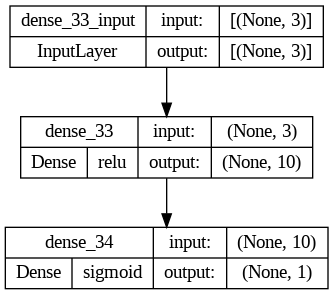
\includegraphics[width=0.3\textwidth]{img/rete/struttura_rete_pca.png}
    \caption{Struttura della rete neurale addestrata con PCA}
    \label{fig:strutturaReteNeuralePCA}
\end{figure}
\subsection{Risultati}
Addestrato il modello con i dati ottenuti attraverso la PCA, si è proceduto con
la valutazione delle prestazioni del modello utilizzando le stesse metriche
utilizzate in precedenza e il test set.

I risultati ottenuti dal modello addestrato con la PCA sono riportati in tabella
\ref{tab:risultatiReteNeuralePCA} e sono confrontati con quelli ottenuti dal
modello addestrato con le feature selezionate manualmente.

\begin{table}[ht]
    \centering
    \begin{tabular}{@{}lccccc@{}}
        \toprule
        \rowcolor[HTML]{EFEFEF}
        \multicolumn{1}{c}{\cellcolor[HTML]{EFEFEF}\textbf{Modello}} & \textbf{Accuratezza} & \textbf{F1} & \textbf{Precision} & \textbf{Recall} \\ \midrule
        Rete senza PCA                                               & 98.80\%              & 98.65\%     & 99.10\%            & 98.65\%         \\
        Rete con PCA                                                 & 98.27\%              & 98.07\%     & 97.92\%            & 98.21\%         \\ \bottomrule
    \end{tabular}
    \caption{Risultati ottenuti dai modelli addestrati con PCA}
    \label{tab:risultatiReteNeuralePCA}
\end{table}

Dai valori riportati nella tabella \ref{tab:risultatiReteNeuralePCA} si può notare
che il modello addestrato con le feature selezionate manualmente ha ottenuto
dei risultati migliori rispetto a quello addestrato con la PCA.

È stata anche calcolata la matrice di confusione per il modello addestrato con
la PCA. La matrice di confusione ottenuta è riportata in figura \ref{fig:matriceConfusioneReteNeuralePCA}.

\begin{figure}[!ht]
    \centering
    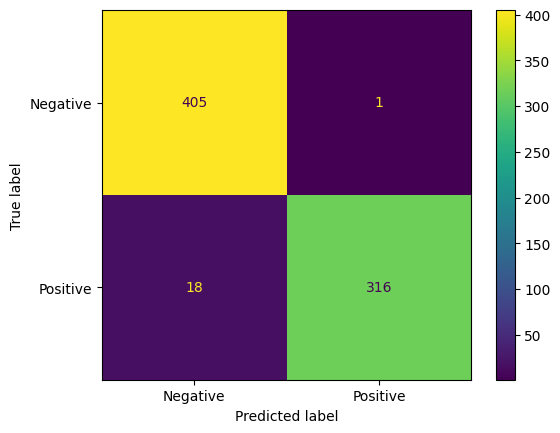
\includegraphics[width=0.5\textwidth]{img/rete/matrice_confusione_pca.png}
    \caption{Matrice di confusione ottenuta dal modello addestrato con PCA}
    \label{fig:matriceConfusioneReteNeuralePCA}
\end{figure}

In aggiunta a queste metriche, i modelli sono stati confrontati attraverso la
10-fold cross validation. I risultati ottenuti sono riportati in tabella
\ref{tab:risultatiCrossValidationPCA}.

\begin{table}[ht]
    \centering
    \resizebox{\textwidth}{!}{\begin{tabular}{@{}lccc@{}}
        \toprule
        \rowcolor[HTML]{EFEFEF}
        \multicolumn{1}{c}{\cellcolor[HTML]{EFEFEF}\textbf{Metrica}} & \textbf{Valore Medio} & \textbf{Intervallo di confidenza con PCA} & \textbf{Intervallo di confidenza senza PCA} \\ \midrule
        Accuratezza                                                  & 98.35 \%              & [97.97\%, 98.72\%]                        & [97.98\%, 98.55\%]                          \\
        Precisione                                                   & 98.05 \%              & [97.51\%, 98.58\%]                        & [97.47\%, 98.52\%]                          \\
        Richiamo                                                     & 98.27 \%              & [97.62\%, 98.93\%]                        & [97.49\%, 98.81\%]                          \\
        F1 score                                                     & 98.15 \%              & [97.73\%, 98.58\%]                        & [97.75\%, 98.38\%]                          \\ \bottomrule
    \end{tabular}}
    \caption{Risultati ottenuti dalla cross validation}
    \label{tab:risultatiCrossValidationPCA}
\end{table}

Oltre a confrontare le performance dei modelli utilizzando le metriche, si
è deciso di confrontare le curve ROC dei due modelli. I risultati ottenuti sono
riportati in figura \ref{fig:confrontoRisultatiPCA}.

\begin{figure}[!ht]
    \centering
    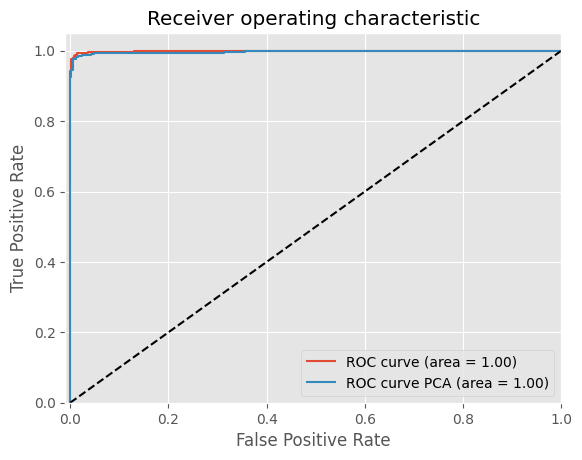
\includegraphics[width=0.8\textwidth]{img/rete/confrontoRoc.png}
    \caption{Confronto curve ROC tra il modello addestrato con e senza PCA}
    \label{fig:confrontoRisultatiPCA}
\end{figure}

Da questa figura si può notare che la differenza tra i due modelli è minima.
Entrambi i modelli si avvicinano molto alla perfetta classificazione. Si può
notare una differenza maggiore tra i due modelli osservando gli intervalli di
confidenza. In particolare, si riesce a osservare una differenza di ampiezza
degli intervalli di confidenza tra i due modelli.

Il modello ottenuto attraverso la PCA ha un intervallo di confidenza più ampio
rispetto a quello ottenuto senza PCA, anche se il valore medio delle metriche
è leggermente superiore nel caso di PCA.

Nella figura \ref{fig:intervalliConfidenzaPCA} sono riportati gli intervalli di
confidenza ottenuti dai modelli addestrati con e senza PCA. Da questa figura si
può notare che l'intervallo di confidenza ottenuto dal modello addestrato con
PCA, rappresentato dalla linea di colore rosso, è più ampio rispetto a quello
ottenuto dal modello addestrato senza PCA, rappresentato dalla linea di colore blu.
\begin{figure}[!ht]
    \centering
    \begin{subfigure}[b]{0.4\textwidth}
        \centering
        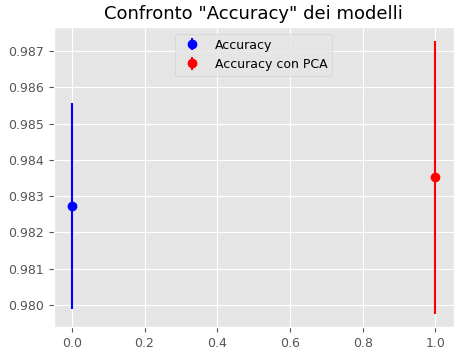
\includegraphics[width=\textwidth]{img/rete/intervalliAcc.png}
        \caption{Accuracy}
        \label{fig:acc}
    \end{subfigure}
    \hfill
    \begin{subfigure}[b]{0.4\textwidth}
        \centering
        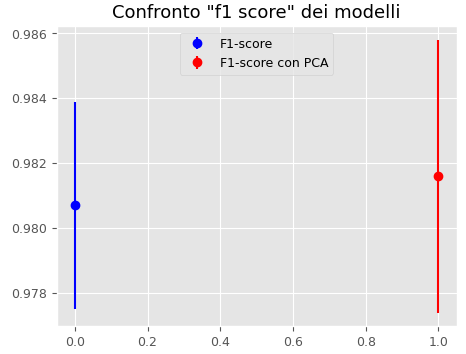
\includegraphics[width=\textwidth]{img/rete/intervalliF1.png}
        \caption{F1 score}
        \label{fig:f1}
    \end{subfigure}
    \hfill
    \begin{subfigure}[b]{0.4\textwidth}
        \centering
        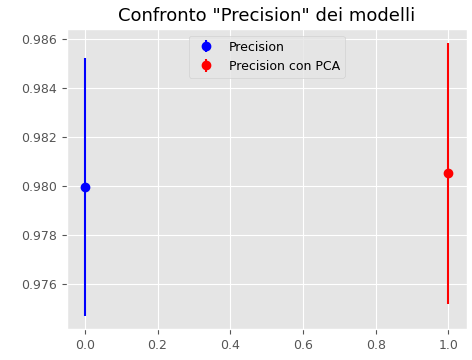
\includegraphics[width=\textwidth]{img/rete/intervalliPrecision.png}
        \caption{Precision}
        \label{fig:precision}
    \end{subfigure}
    \hfill
    \begin{subfigure}[b]{0.4\textwidth}
        \centering
        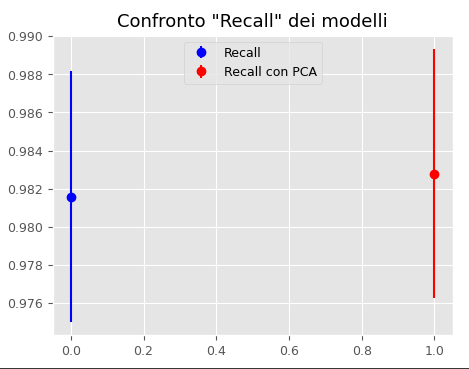
\includegraphics[width=\textwidth]{img/rete/intervalliRecall.png}
        \caption{Recall}
        \label{fig:recall}
    \end{subfigure}
    \caption{Intervalli di confidenza ottenuti dai modelli addestrati con e senza PCA}
    \label{fig:intervalliConfidenzaPCA}
\end{figure}
